\documentclass[13pt,oneside]{book}
\usepackage[utf8]{inputenc}
\usepackage{url}
\usepackage{listings}
\usepackage{graphicx}

\usepackage{geometry}
\geometry{a4paper, left=20mm, right=20mm, top=20mm, bottom=20mm}
\usepackage[margin=1.2in]{geometry}
\usepackage[toc,page]{appendix}
\usepackage{graphicx}
\usepackage{natbib}
\usepackage{lipsum}
\usepackage{caption}

\begin{document}

\captionsetup[figure]{margin=1.5cm,font=small,labelfont={bf},name={Figure},labelsep=colon,textfont={it}}
\captionsetup[table]{margin=1.5cm,font=small,labelfont={bf},name={Table},labelsep=colon,textfont={it}}
\setlipsumdefault{1}

\begin{titlepage}
\begin{center}
{\LARGE College Of Engineering Trivandrum}\\[3cm]
\linespread{1.2}\huge {\bfseries System Software Lab}\\[3cm]
\linespread{1}

\includegraphics[width=5cm]{img/emblem.jpeg}\\[3cm]
{\Large GOKUL K\\ S5  CSE \\ Roll No:21\\ TVE18CS021 }\\[1cm]


\textit{ }\\[2cm]
Department of Computer Science\\[0.2cm]
\today
\end{center}

\end{titlepage}

\newpage

\begin{frame}{}
    \centering
    \hspace*{-0.5cm}
    $\vcenter{\hbox{
\includegraphics[width=1.5cm]{img/emblem.jpeg}}}$
    $\vcenter{\resizebox{0.95\textwidth}{!}{
        \begin{tabular}{c}
             CS331 - System Software Lab $\cdot$ 2020 $\cdot$   \\
             \hline 
        \end{tabular}
    }}$
\end{frame}
\section*{Cycle 2}
\section*{Expt 5}
\begin{center}
    \Large{Implementation of Absolute Loader}
\end{center}
\section*{Aim}
\large
To implement an absolute loader

\section*{Algorithm} 
    \begin{verbatim}
1 begin
2 read Header record
3 verify program name and length
4 read first Text record
5 while record type != E do
6 begin
7 {if object code is in character form , convert into
8 internal representation }
9 move object code to specified location in memory
10 read next object program record
11 end
12 jump to address specified in End record
13 end
	\end{verbatim}

\section*{Source Code}
\small

\begin{lstlisting}[language=C]
/*  Implement an absolute loader */
#include <stdio.h>
#include <stdlib.h>
#include <string.h>

int main()
{
	FILE * objcode, * output;
	char prgrm_name[20], prgrm_name_in_file[20], * token;
	char code, start_addr[20], total[20], line[50]; 
	int i, start_addri;

	if(! (objcode = fopen("objcode.txt", "r")))
	{
		printf("Please save the object code as objcode.txt");
		exit(0);
	}

	printf("Enter program name: ");
	scanf("%s", prgrm_name);

	// Reading the header record
	fscanf(objcode, "%c^%s", &code, line);
	strcpy(prgrm_name_in_file, strtok(line, "^"));

	// Verifying program name
	if(strcmp(prgrm_name, prgrm_name_in_file) != 0)
	{
		printf("Program name does not match\n");
		exit(0);
	}
	
	while(! feof(objcode))
	{
		fscanf(objcode, "%c^%s", &code, line);
		switch (code)
		{
			case 'T':
				strcpy(start_addr, strtok(line, "^"));
				start_addri = atoi(start_addr);
				
				// Ignoring the length string
				token = strtok(NULL, "^");
				token = strtok(NULL, "^");

				while(token != NULL)
				{
					for(i = 0; i < strlen(token); i += 2)
					{
						printf(
							"%d %c%c\n", 
							start_addri, 
							token[i], 
							token[i+1]
						);
						++start_addri;
					}

					token = strtok(NULL, "^");
				}
				break;
			
			case 'E':
				fclose(objcode);
				return 0;
		}
	}
}	
    \end{lstlisting}
    \section*{Output}
    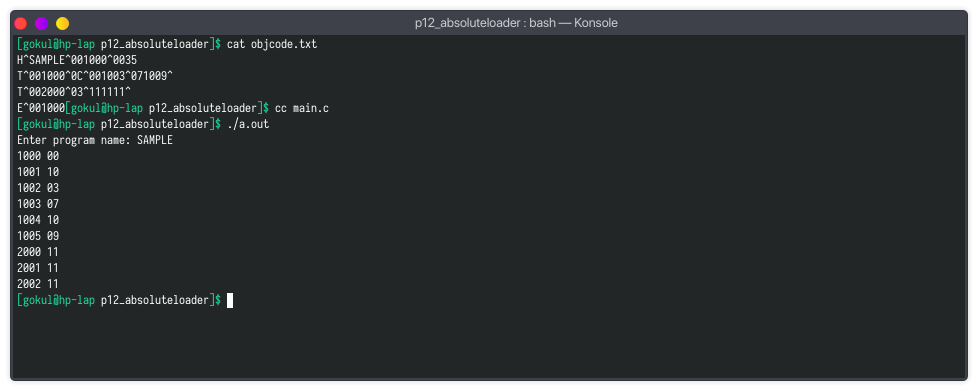
\includegraphics[width=\textwidth]{img/p12.png}
     
\Large
\section*{Result}
\large
Absolute loader is implemented and its output is verified
\end{document}